% Slides2_Comet.tex

\documentclass[10pt, a4paper]{beamer}



\usepackage{amsmath , amssymb , amsthm}
\usepackage{graphicx , float}
\usepackage{layout}
\usepackage{caption, subcaption}


\title     {Slides2}
\author{Andrea Boselli}
\date{\today}



\begin{document}
	
	
	\begin{frame} {A. Comet Equation}
		
		It's a linear advection-diffusion PDE, featuring 2 parameters, each with a clear physical interpretation:
		
		\begin{equation*}
			\begin{cases}
				- \mu \Delta u + 10(\text{cos}\theta, \text{sin}\theta) \cdot \nabla u = 10 e^{-50 \| \underline{x} - \underline{x}_{0}  \|_2   } \quad\quad & \underline{x} \in \Omega = \left[0,1\right]^2\\
				u = 0 & \underline{x} \in \partial \Omega
			\end{cases}	
		\end{equation*}
	
		\begin{itemize}
			
			\item $\mu \in (0,\infty)$: diffusion parameter
			\item $\theta \in (0,2\pi)$: angle of advection term
			\item$\underline{x}_0 = (0.5,0.5)$: centre of the forcing bump
			
		\end{itemize}
		
		\vspace{\baselineskip}
		Data is produced through simulation with fixed and known values of parameters and error scale:
	
		\begin{center}
			$\mu^* = 2$ \hspace{2cm} $\theta^* = \pi$ \hspace{2cm} $\tau^* = 10^{-4}$
		\end{center}
		
	\end{frame}





	\begin{frame}{A1. Comet with Different Grids}
		
		\vspace{0.5\baselineskip}
		
		$u(\underline{\theta}, \underline{x})$ is approximated through Finite Element Method (FEM). The mesh refinement affects the accuracy of the numerical solution.
		
		\vspace{0.5\baselineskip}
			
		 In MLDA, coarse and fine model differ for the mesh refinement.
		
		\vspace{0.5\baselineskip}

		Comparison of:
		
		\begin{itemize}
			
			\item Metropolis: 32x32 elements
			
			\item MLDA
			
			\begin{itemize}
				
				\item Coarse model: 16x16 elements
				
				\item Fine model: \hspace{2mm} 32x32 elements
				
			\end{itemize}
			
		\end{itemize}
		
		\begin{figure}[H]
			
			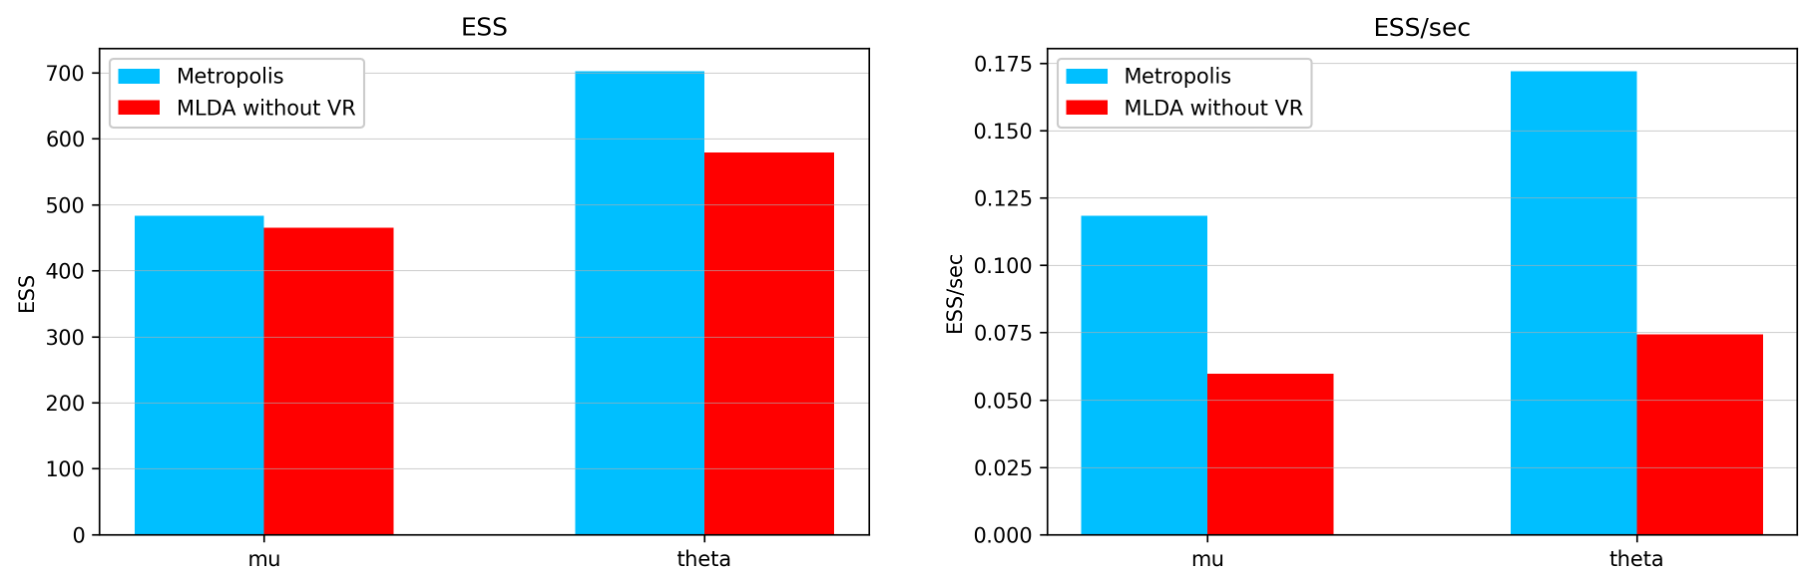
\includegraphics[height= 3.5cm, keepaspectratio]{A1_ESS_Comparison}
			
		\end{figure}
		
	\end{frame}





	\begin{frame}{A1. Comet with Different Grids}
		
		\vspace{0.5\baselineskip}
		
		$u(\underline{\theta}, \underline{x})$ is approximated through Finite Element Method (FEM). The mesh refinement affects the accuracy of the numerical solution.
		
		\vspace{0.5\baselineskip}
		
		In MLDA, coarse and fine model differ for the mesh refinement.
		
		\vspace{0.5\baselineskip}
		
		Comparison of:
		
		\begin{itemize}
			
			\item Metropolis: 32x32 elements
			
			\item MLDA
			
			\begin{itemize}
				
				\item Coarse model: 16x16 elements
				
				\item Fine model: \hspace{2mm} 32x32 elements
				
			\end{itemize}
			
		\end{itemize}
		
		\begin{figure}[H]
			
			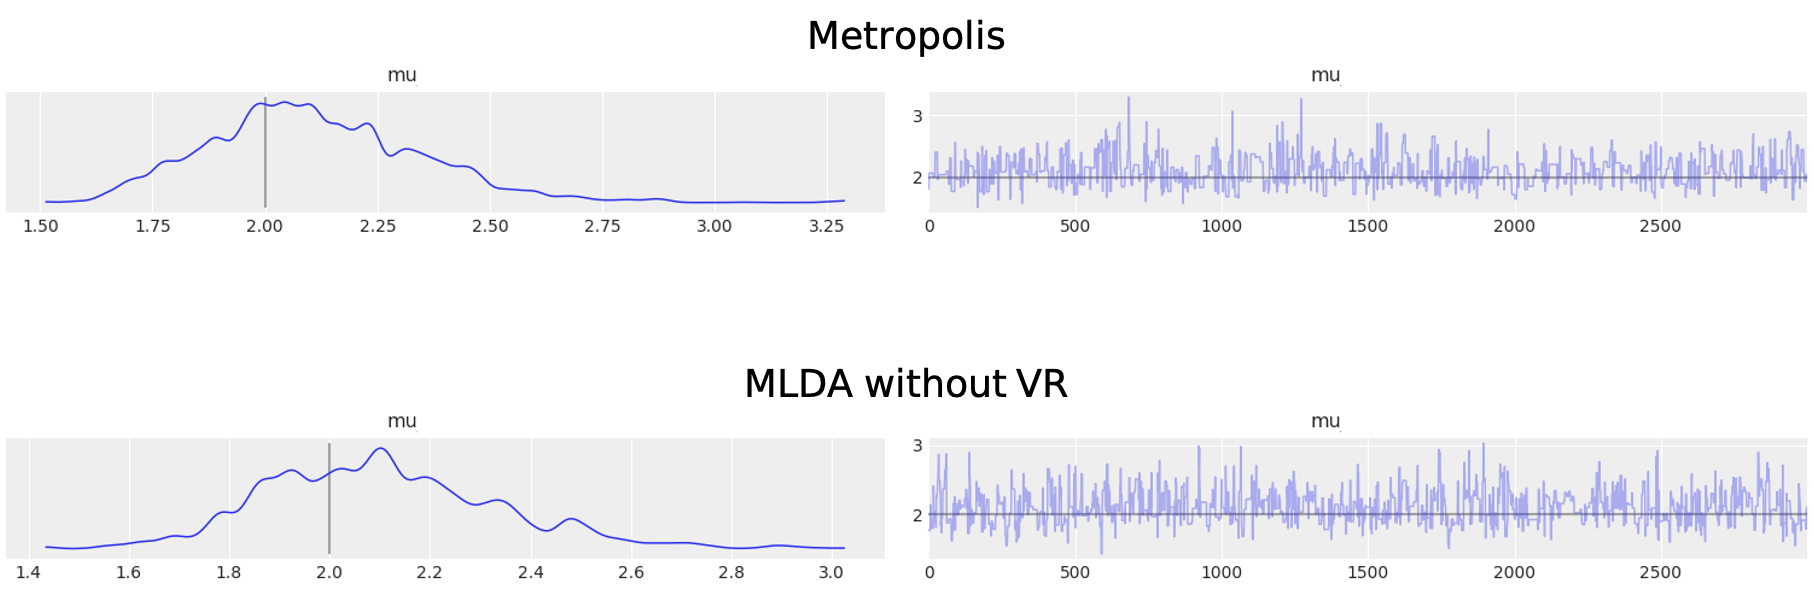
\includegraphics[height= 3.5cm, keepaspectratio]{A1_Metropolis_MLDA}
			
		\end{figure}
		
	\end{frame}

	\begin{frame}{A2. Comet with Surrogate Model}
		
		Metropolis overcomes MLDA evidently. Indeed, coarse solution in MLDA is too time consuming. \\
		
		Hence, we place at coarse level a surrogate model, implemented through a Neural Network:
		
		\begin{equation*}
			u_{\text{NN}}: (\mu,\theta,x,y) \mapsto u_{\text{NN}}(\mu,\theta,x,y)
		\end{equation*}
	
		\begin{figure}[H]
			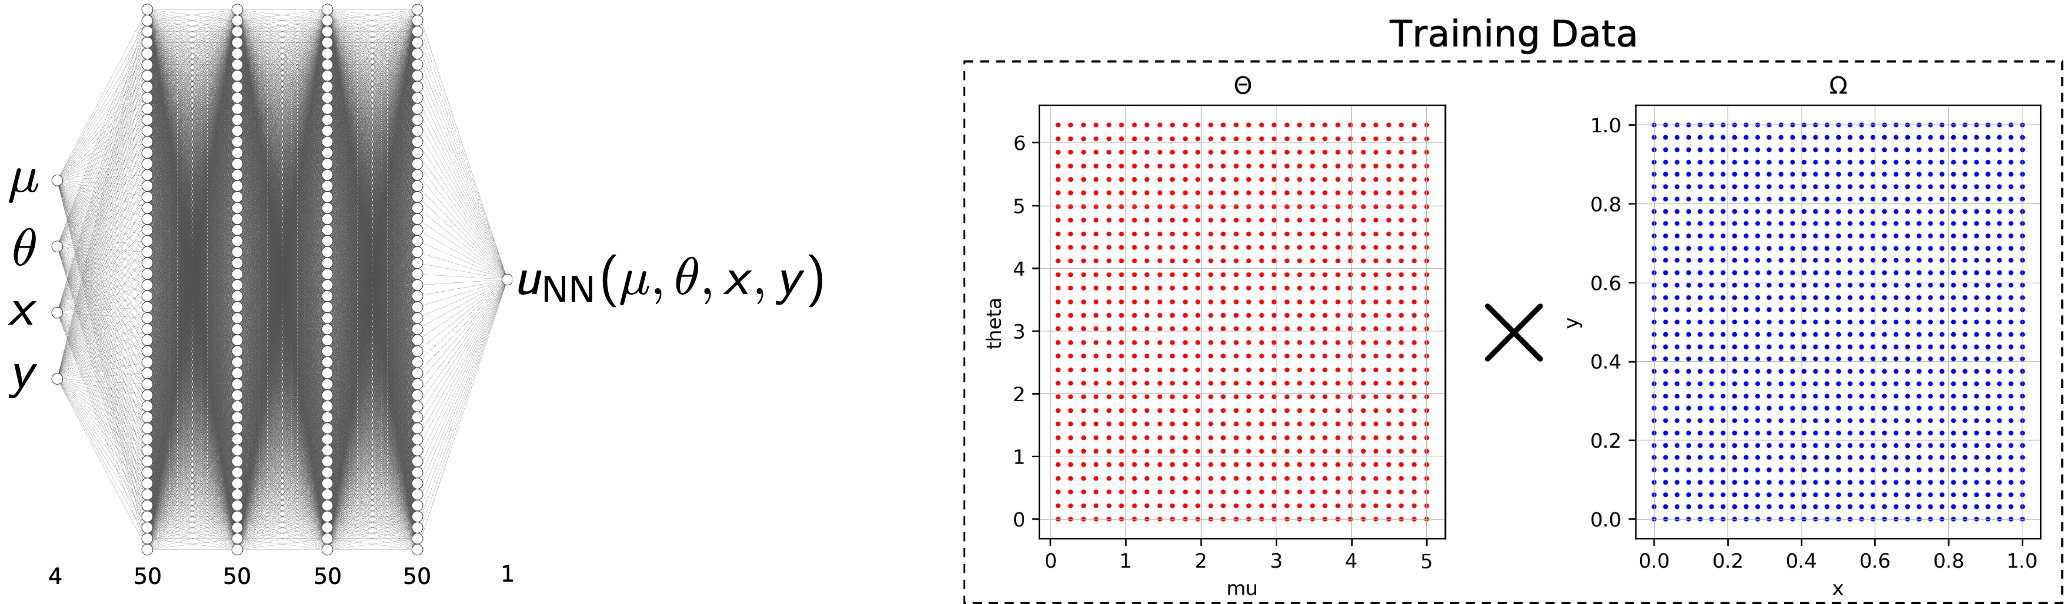
\includegraphics[height = 3.1cm]{Surrogate_Images}
		\end{figure}

		$u_{\text{NN}}$ is trained on a dataset of 900 PDE solutions (each corresponding to a different $(\mu_i,\theta_i)$), evaluated on a grid of $\Omega$
	
		\begin{center}
			+ Long training time	 \hspace{2cm}	- Small execution time
		\end{center}
		
	\end{frame}

	\begin{frame}{A2. Comet with Surrogate Model}
		
		Within this framework, we investigated the performances of Metropolis, DEMetropolisZ and MLDA for different:
		
		\begin{itemize}
			
			\item frequencies of subsampling (nsubs) of proposed samples from coarse level to fine level in MLDA
			\item grids of physical points where data is available
			\item choices of the priors for $(\mu,\theta)$
			
		\end{itemize}
		
		\vspace{0.5\baselineskip}
	
		Comparison of Metropolis, DEMetropolisZ and MLDA (nsubs = 5, 20):
	
		\begin{figure}[H]
			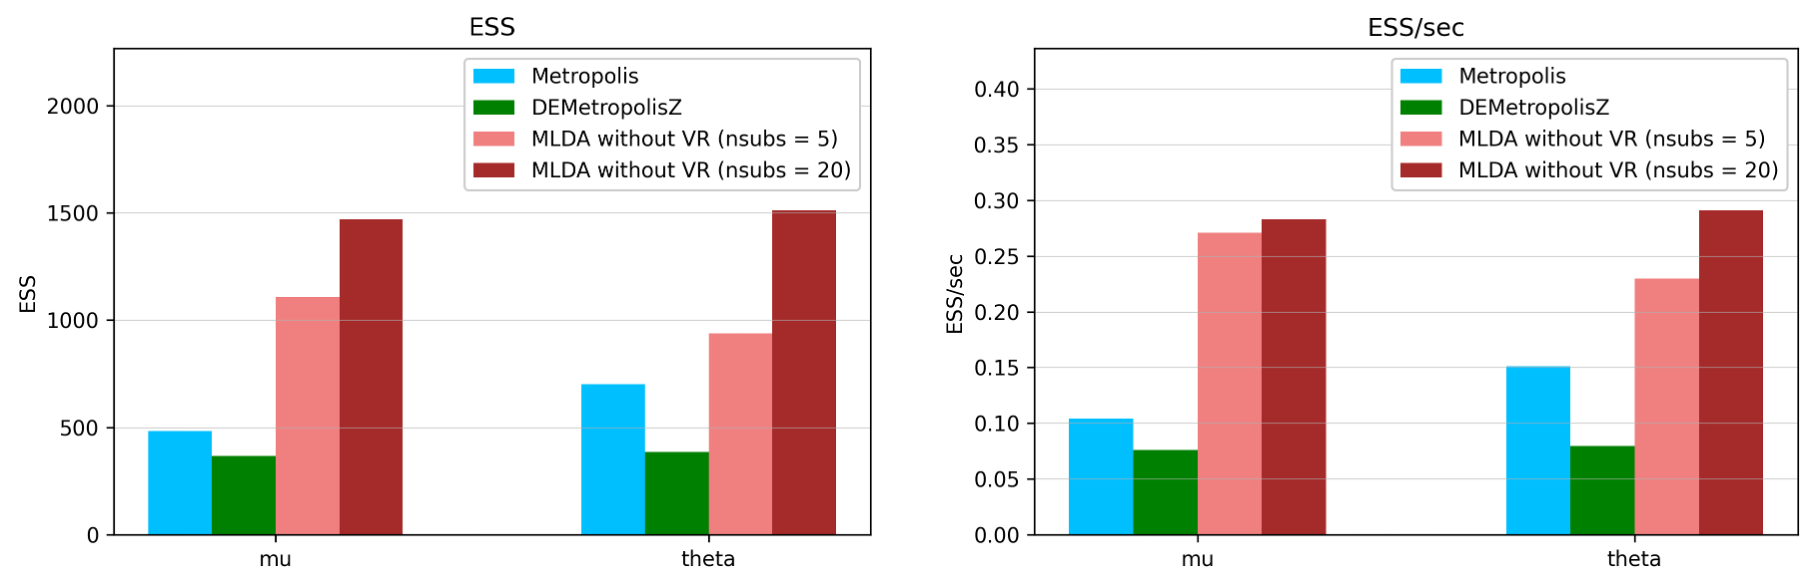
\includegraphics[height = 3.5cm]{A2_ESS_Comparison}
		\end{figure}
		
	\end{frame}

	\begin{frame}{A2. Comet with Surrogate Model}
		
		Comparison of Metropolis, DEMetropolisZ and MLDA (nsubs = 5, 20):

		\begin{figure}[H]
			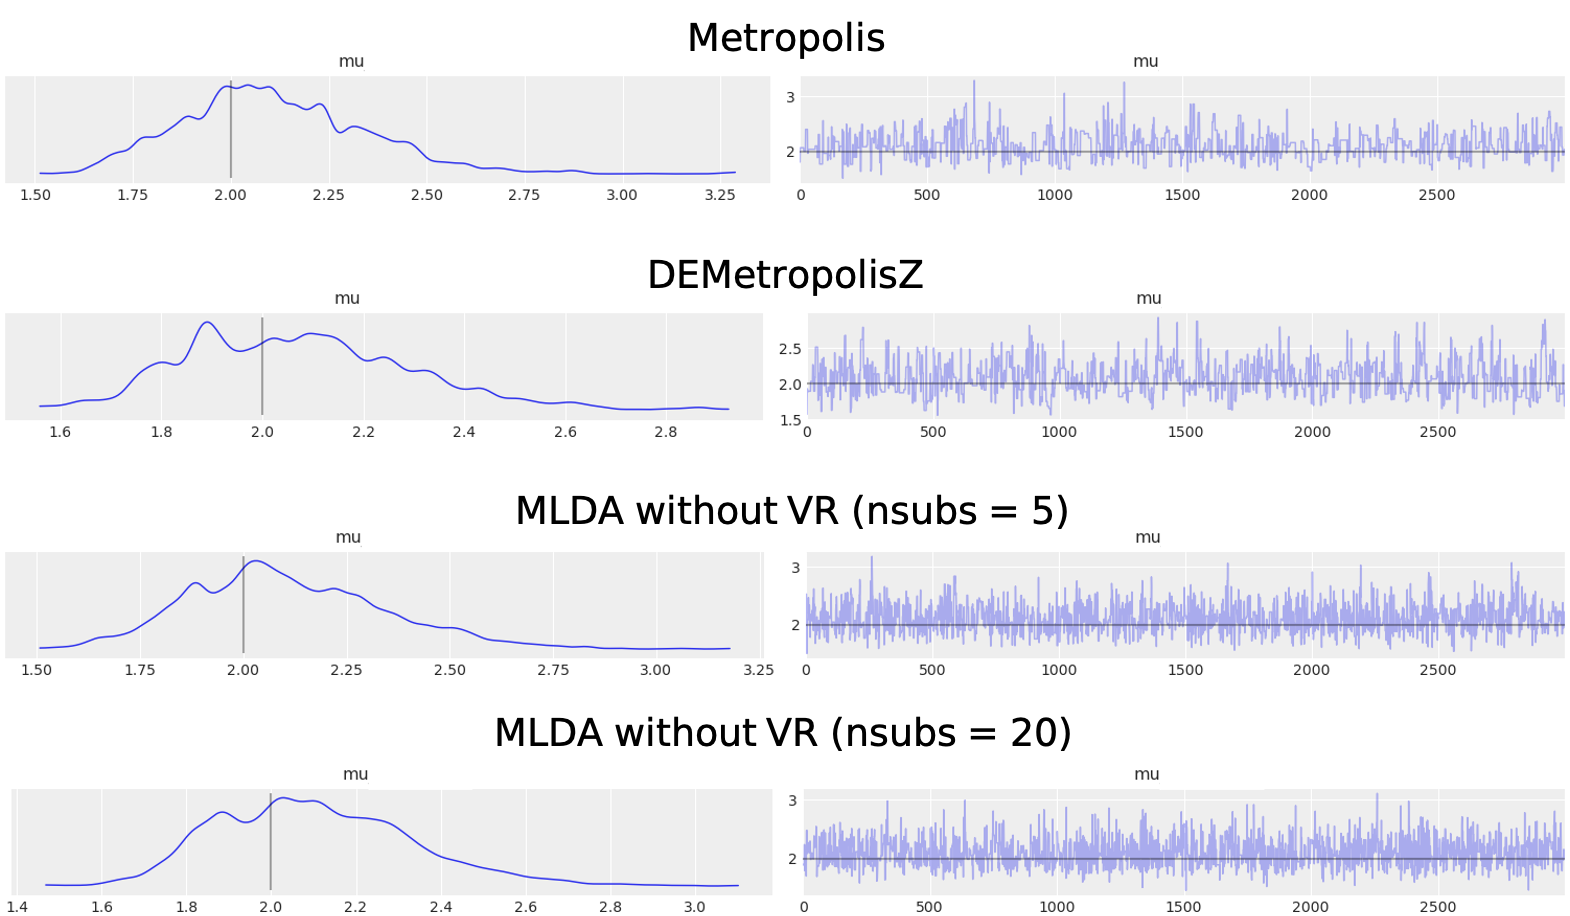
\includegraphics[height = 6.5cm]{A2_Traceplots}
		\end{figure}

	\end{frame}
	
\end{document}